\documentclass[border=5mm]{standalone}
\usepackage{tikz}
\usetikzlibrary{positioning}
\begin{document}
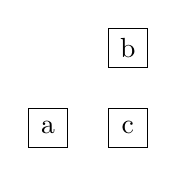
\begin{tikzpicture}[
  every node/.style={draw, rectangle, minimum size=5mm},
  node distance=5mm,
]

% \node (a) {a};
% \node (b) [right=of a] {b};
% \node (c) [red, above right=of a] {c};
% \node (c) [green, above right=5mm and 5mm of a] {c};
% \node (c) [blue, above right=5mm and 0mm of a] {c};

\node (a) {a};
\node (b) [above right=5mm and 5mm of a] {b};
% \node (c) at ((a) -| (b)) {c};
\path (a -| b) node {c};


\end{tikzpicture}
\end{document}